\documentclass[tikz,border=5pt]{standalone}
\usepackage{amsmath}
\usetikzlibrary{arrows.meta,positioning,calc}

\definecolor{siteaccent}{RGB}{54,117,138}
\definecolor{sitelight}{RGB}{238,245,247}
\definecolor{siteborder}{RGB}{190,211,218}
\definecolor{sitetext}{RGB}{32,39,43}
\definecolor{sitemuted}{RGB}{102,116,123}

\tikzset{
  block/.style={draw=siteborder, fill=sitelight, rounded corners=2pt,
    minimum height=12mm, align=center, inner xsep=5pt, text=sitetext},
  result/.style={draw=siteaccent, fill=white, rounded corners=2pt,
    minimum height=10mm, align=center, inner xsep=5pt, text=sitetext},
  flow/.style={-{Latex[length=2.2mm]}, semithick, draw=siteaccent},
  sample/.style={circle, fill=siteaccent, inner sep=1.6pt}
}

\begin{document}
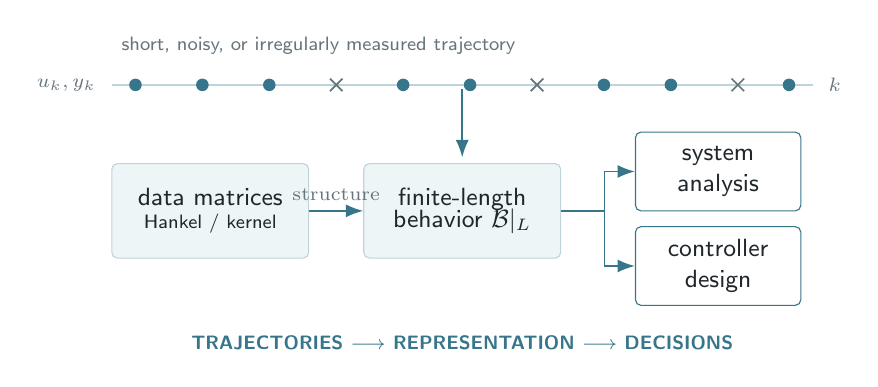
\begin{tikzpicture}[font=\sffamily\small]
  % Irregularly measured trajectory
  \node[anchor=west, text=sitemuted, font=\sffamily\scriptsize] at (0,2.85)
    {short, noisy, or irregularly measured trajectory};
  \draw[siteborder, semithick] (0,2.35) -- (8.9,2.35);
  \foreach \x in {0.3,1.15,2.0,3.7,4.55,6.25,7.1,8.6}
    \node[sample] at (\x,2.35) {};
  \foreach \x in {2.85,5.4,7.95} {
    \draw[sitemuted, semithick] (\x-0.08,2.27) -- (\x+0.08,2.43);
    \draw[sitemuted, semithick] (\x-0.08,2.43) -- (\x+0.08,2.27);
  }
  \node[anchor=east, text=sitemuted, font=\sffamily\scriptsize] at (-0.08,2.35) {$u_k,y_k$};
  \node[anchor=west, text=sitemuted, font=\sffamily\scriptsize] at (8.98,2.35) {$k$};

  \node[block, minimum width=25mm] (data) at (1.25,0.75)
    {data matrices\\[-1mm]\scriptsize Hankel / kernel};
  \node[block, minimum width=25mm] (behavior) at (4.45,0.75)
    {finite-length\\[-1mm]behavior $\mathcal{B}|_L$};
  \node[result, minimum width=21mm] (analysis) at (7.7,1.25)
    {system\\analysis};
  \node[result, minimum width=21mm] (control) at (7.7,0.05)
    {controller\\design};

  \draw[flow] (4.45,2.3) -- (4.45,1.43);
  \draw[flow] (data) -- node[above, text=sitemuted, font=\scriptsize] {structure} (behavior);
  \draw[flow] (behavior.east) -- ++(0.55,0) |- (analysis.west);
  \draw[flow] (behavior.east) -- ++(0.55,0) |- (control.west);

  \node[anchor=north, text=siteaccent, font=\sffamily\scriptsize\bfseries]
    at (4.45,-0.72) {TRAJECTORIES $\longrightarrow$ REPRESENTATION $\longrightarrow$ DECISIONS};
\end{tikzpicture}
\end{document}
